\subsection*{Méthodologie}
Les mortgages backed securities ou titres adossés à des créances hypo\-thécaires sont un
type d'obli\-gation adossé à des actifs, sécurisé par un pool d'hypothèques. Des banques
d'investis\-sements achètent les hypothèques et titrisent les prêts hypothecaires afin de
les revendre à des investisseurs.  Un facteur à prendre en compte lorsqu'il est question
d'évaluer une MBS est la vitesse de prépaiement des débiteurs hypothécaires. En effet,
selon le niveau de taux d'intérêt, les détenteurs d'hypothèques repaient leur dette plus
ou moins rapidement. Pour intégrer cet aspect à l'évaluation de la MBS, nous attribuons
une probabilité de prépaiement $p_t$ pour chaque mensualité $t$. Cette probabilité
correspond à une fonction intégrant un facteur de taux de prépaiement conditionel, dénoté
ici par $CPR_t$ (conditional prepayment rate). Le $CPR_t$ est définit dans le mandat par
la fonction suivante:
\[
CPR_t= 0.07+1.05*\max\{(0.0594-(0.00837+0.905r_t),0\}
\]
dont les valeurs sont fondées sur les travaux de \cite{chernov2016macroeconomic}.

La probabilité $p_t$ est ensuite déterminée comme suit: 
\[
p_t=1-(1-CPR_t)^{1/12}
\]
et illustre la vitesse à laquelle le prepaiement survient. 

Les cashflows de la MBS se résument aux trois quantités suivantes:
\begin{gather*}
\text{Paiement d'intérêts sur MBS}: I_t^{MBS}=\frac{r_{12}^{MBS}}{12}*L_t \\
\text{Principal anticipé}: Pay_t^{scheduled}=C_t-I_t \\
\text{Prepaiement du principal}: Pay_t^{prepaid}=p_t*L_t
\end{gather*}
et requièrent les quantités ci-dessous:
\begin{gather*}
\text{Paiement d'intérêts hypothécaires:} I_t=\frac{r_{12}^{m}}{12}*L_t \\
\text{Principal non-payé}: L_{t+1}=L_t-Pay_t^{scheduled}-Pay_t^{prepaid} \\
\text{Mise à jour du coupon anticipé}: C_{t+1}=(1-p_t)*C_t
\end{gather*}

Le coupon initial $C_0$ est déterminé de façon à satisfaire la relation de la valeur actualisée des coupons et du principal définie par
\[
\text{Principal}=\sum_{i=1}^{5\cdot 12} \frac{C_0}{\left(1+\frac{r_{12}^{m}}{12}\right)^i}
\]

La valeur du Principal
$L_0$ correspond à la valeur indiquée dans le descriptif de la MBS dans le mandat,
c'est-à-dire \num{7326596}\$.

Ainsi nous pouvons définir le flux monétaire mensuel généré par la MBS selon:
\[
\text{Cash-flow total par mensualité}: CF_t=I_t+Pay_t^{scheduled}+Pay_t^{prepaid}.
\]


Les dérivés hypothécaires \textit{Interest Only strips} et \textit{Principal Only strips}
que le courtier souhaite émettre constituent les flux monétaires d'une MBS lorsqu'ils sont
combinés. La \textit{Interest Only} verse à son détenteur les flux monétaires attachés aux
coupons de la mortgage backed security. Le détenteur d'une IO est long le taux d'intêret
puisqu'une baisse du taux incite les détenteurs d'hypothèques à accélérer le remboursement
de leurs hypothèques. Par conséquent, les intérêts de la MBS sont perçus sur un capital
qui décroît plus vite. À l'inverse, la \textit{Principal only} découle des flux monétaires
liés au remboursement du principal et celle-ci prend de la valeur lorsque le taux
d'intêret baisse, puisque il accélère le remboursement des hypothèques et donc des flux
monétaires de la PO.

\small
\begin{table}
  \centering
  \caption{}
  \label{mbs_table}
  \makebox[\textwidth]{\begin{tabular}{lrrrrrrr}
\toprule
{} &          $p$ &            Coupon &          Principal &   Princ. anticipé &   Int. transféré &   Princ. prépayé &             Int. \\
\midrule
0  & \num{0.0109} & \num{139861.29}\$ & \num{7326596.00}\$ & \num{103655.69}\$ & \num{33580.23}\$ & \num{79998.34}\$ & \num{36205.60}\$ \\
1  & \num{0.0105} & \num{138396.26}\$ & \num{7142941.97}\$ & \num{103098.22}\$ & \num{32738.48}\$ & \num{74821.44}\$ & \num{35298.04}\$ \\
2  & \num{0.0104} & \num{136950.19}\$ & \num{6965022.32}\$ & \num{102531.37}\$ & \num{31923.02}\$ & \num{72775.54}\$ & \num{34418.82}\$ \\
3  & \num{0.0107} & \num{135486.35}\$ & \num{6789715.40}\$ & \num{101933.84}\$ & \num{31119.53}\$ & \num{72574.37}\$ & \num{33552.51}\$ \\
4  & \num{0.0105} & \num{134067.52}\$ & \num{6615207.18}\$ & \num{101377.37}\$ & \num{30319.70}\$ & \num{69275.38}\$ & \num{32690.15}\$ \\
5  & \num{0.0107} & \num{132638.05}\$ & \num{6444554.43}\$ & \num{100791.21}\$ & \num{29537.54}\$ & \num{68713.93}\$ & \num{31846.84}\$ \\
6  & \num{0.0105} & \num{131241.82}\$ & \num{6275049.30}\$ & \num{100232.62}\$ & \num{28760.64}\$ & \num{66054.79}\$ & \num{31009.20}\$ \\
7  & \num{0.0107} & \num{129834.85}\$ & \num{6108761.88}\$ &  \num{99647.39}\$ & \num{27998.49}\$ & \num{65488.46}\$ & \num{30187.46}\$ \\
8  & \num{0.0102} & \num{128507.03}\$ & \num{5943626.03}\$ &  \num{99135.61}\$ & \num{27241.62}\$ & \num{60785.60}\$ & \num{29371.42}\$ \\
9  & \num{0.0107} & \num{127126.66}\$ & \num{5783704.82}\$ &  \num{98545.52}\$ & \num{26508.65}\$ & \num{62126.30}\$ & \num{28581.14}\$ \\
10 & \num{0.0103} & \num{125810.98}\$ & \num{5623033.00}\$ &  \num{98023.83}\$ & \num{25772.23}\$ & \num{58194.71}\$ & \num{27787.15}\$ \\
11 & \num{0.0101} & \num{124536.75}\$ & \num{5466814.47}\$ &  \num{97521.57}\$ & \num{25056.23}\$ & \num{55368.85}\$ & \num{27015.17}\$ \\
12 & \num{0.0094} & \num{123361.96}\$ & \num{5313924.05}\$ &  \num{97102.32}\$ & \num{24355.49}\$ & \num{50127.42}\$ & \num{26259.64}\$ \\
13 & \num{0.0100} & \num{122126.62}\$ & \num{5166694.31}\$ &  \num{96594.54}\$ & \num{23680.68}\$ & \num{51739.05}\$ & \num{25532.08}\$ \\
14 & \num{0.0107} & \num{120819.70}\$ & \num{5018360.72}\$ &  \num{96020.63}\$ & \num{23000.82}\$ & \num{53703.34}\$ & \num{24799.07}\$ \\
15 & \num{0.0103} & \num{119571.10}\$ & \num{4868636.74}\$ &  \num{95511.92}\$ & \num{22314.59}\$ & \num{50314.29}\$ & \num{24059.18}\$ \\
16 & \num{0.0097} & \num{118415.24}\$ & \num{4722810.53}\$ &  \num{95076.68}\$ & \num{21646.21}\$ & \num{45654.27}\$ & \num{23338.56}\$ \\
17 & \num{0.0096} & \num{117281.87}\$ & \num{4582079.57}\$ &  \num{94638.76}\$ & \num{21001.20}\$ & \num{43855.83}\$ & \num{22643.11}\$ \\
18 & \num{0.0097} & \num{116147.35}\$ & \num{4443584.98}\$ &  \num{94188.64}\$ & \num{20366.43}\$ & \num{42984.56}\$ & \num{21958.72}\$ \\
19 & \num{0.0101} & \num{114971.57}\$ & \num{4306411.78}\$ &  \num{93690.72}\$ & \num{19737.72}\$ & \num{43594.54}\$ & \num{21280.85}\$ \\
20 & \num{0.0105} & \num{113762.64}\$ & \num{4169126.52}\$ &  \num{93160.21}\$ & \num{19108.50}\$ & \num{43838.56}\$ & \num{20602.43}\$ \\
21 & \num{0.0101} & \num{112611.97}\$ & \num{4032127.76}\$ &  \num{92686.54}\$ & \num{18480.59}\$ & \num{40783.50}\$ & \num{19925.43}\$ \\
22 & \num{0.0095} & \num{111543.35}\$ & \num{3898657.71}\$ &  \num{92277.48}\$ & \num{17868.85}\$ & \num{36996.09}\$ & \num{19265.87}\$ \\
23 & \num{0.0091} & \num{110530.44}\$ & \num{3769384.14}\$ &  \num{91903.40}\$ & \num{17276.34}\$ & \num{34229.15}\$ & \num{18627.04}\$ \\
24 & \num{0.0090} & \num{109538.32}\$ & \num{3643251.58}\$ &  \num{91534.58}\$ & \num{16698.24}\$ & \num{32701.98}\$ & \num{18003.73}\$ \\
25 & \num{0.0089} & \num{108561.34}\$ & \num{3519015.02}\$ &  \num{91171.54}\$ & \num{16128.82}\$ & \num{31386.20}\$ & \num{17389.80}\$ \\
26 & \num{0.0085} & \num{107641.81}\$ & \num{3396457.28}\$ &  \num{90857.65}\$ & \num{15567.10}\$ & \num{28768.46}\$ & \num{16784.16}\$ \\
27 & \num{0.0080} & \num{106784.64}\$ & \num{3276831.17}\$ &  \num{90591.64}\$ & \num{15018.81}\$ & \num{26093.93}\$ & \num{16193.01}\$ \\
28 & \num{0.0068} & \num{106055.94}\$ & \num{3160145.60}\$ &  \num{90439.55}\$ & \num{14484.00}\$ & \num{21564.96}\$ & \num{15616.39}\$ \\
29 & \num{0.0074} & \num{105273.81}\$ & \num{3048141.08}\$ &  \num{90210.91}\$ & \num{13970.65}\$ & \num{22479.17}\$ & \num{15062.90}\$ \\
30 & \num{0.0072} & \num{104518.86}\$ & \num{2935451.00}\$ &  \num{90012.84}\$ & \num{13454.15}\$ & \num{21050.91}\$ & \num{14506.02}\$ \\
31 & \num{0.0069} & \num{103802.24}\$ & \num{2824387.25}\$ &  \num{89845.06}\$ & \num{12945.11}\$ & \num{19365.05}\$ & \num{13957.18}\$ \\
32 & \num{0.0066} & \num{103117.17}\$ & \num{2715177.15}\$ &  \num{89699.67}\$ & \num{12444.56}\$ & \num{17919.53}\$ & \num{13417.50}\$ \\
33 & \num{0.0060} & \num{102495.45}\$ & \num{2607557.95}\$ &  \num{89609.76}\$ & \num{11951.31}\$ & \num{15721.77}\$ & \num{12885.68}\$ \\
34 & \num{0.0060} & \num{101877.47}\$ & \num{2502226.41}\$ &  \num{89512.30}\$ & \num{11468.54}\$ & \num{15086.69}\$ & \num{12365.17}\$ \\
35 & \num{0.0060} & \num{101263.22}\$ & \num{2397627.42}\$ &  \num{89414.94}\$ & \num{10989.13}\$ & \num{14456.03}\$ & \num{11848.28}\$ \\
\bottomrule
\end{tabular}
}
\end{table}
\normalsize

Pour obtenir la valeur de la IO, il suffit de faire la somme de tous les cashflows
d'intérêt payés par la MBS (colonne 6), ajustés par le facteur d'actualisation
correspondant à la période $t$ (colonne 9). La valeur de la PO est constituée de la somme
des paiements anticipés (colonne 8) actualisés ainsi que la somme des prépaiements de
principal (colonne 5) actualisés.



\subsection*{Résultats}
La Table \ref{iopo_table} présente les prix obtenus, ainsi que les statistiques associées,
pour une évaluation Monte Carlo de \num{50000} trajectoires. En outre, la Figure
\ref{histos} présente un histogramme de la valeur des IO et des PO. On remarque notamment
l'asymétrie opposée des deux produits dérivés.

Pour expliquer ces résultats, attardons nous d'abord sur l'histogramme de la valeur des
IO. On remarque que celle-ci suit de près la distribution des taux courts. Mais la valeur
d'un dérivé IO est directement corrélé à la valeur des taux courts: des taux élevés
impliquent un prépaiement faible, et donc un principal plus important sur lequel prélever
des intérêts. Et inversement pour les taux faibles.

De la même façon, des taux élevés impliquent une hausse dans les prépaiements ce qui
entraîne alors des flux monétaires importants et donc hausse la valeur du PO, ce qui
explique une distribution symétrique à celles des taux courts. 

\begin{figure}
  \centering
  \begin{subfigure}{0.3\paperwidth}
    \centering
    \caption{Histogramme de la valeur des PO}
    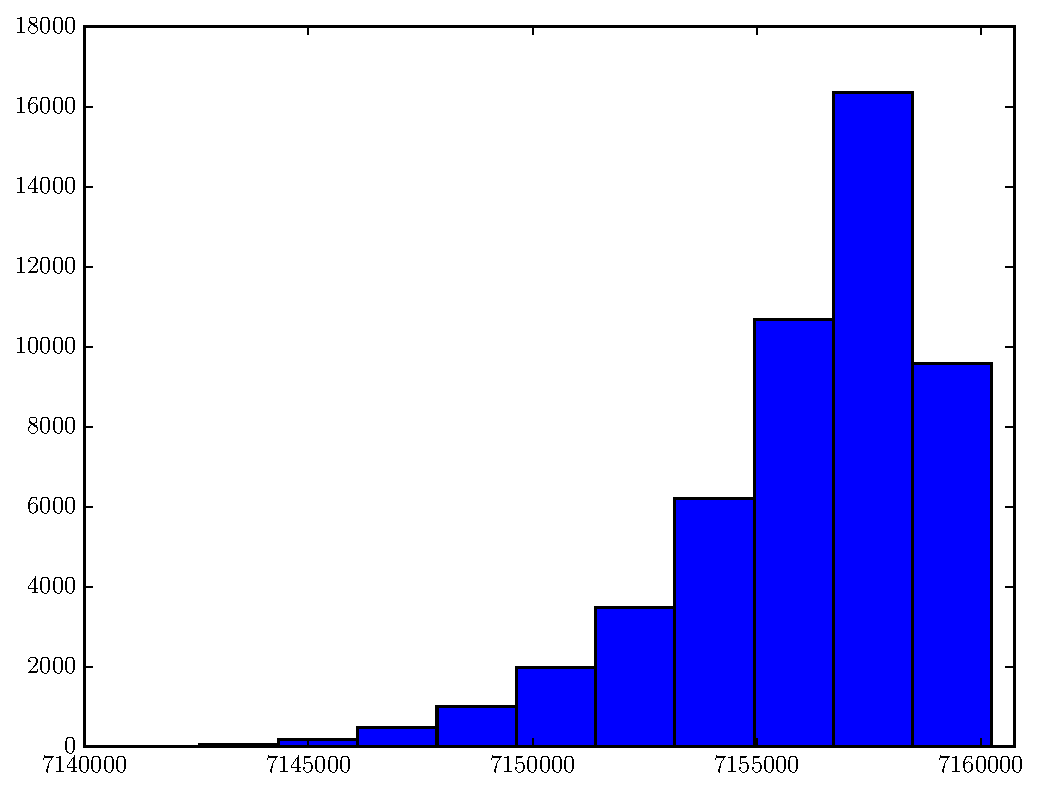
\includegraphics[width=0.3\paperwidth]{../fig/po_hist.pdf}
  \end{subfigure}
  ~
  \begin{subfigure}{0.3\paperwidth}
    \centering
    \caption{Histogramme de la valeur des IO}
    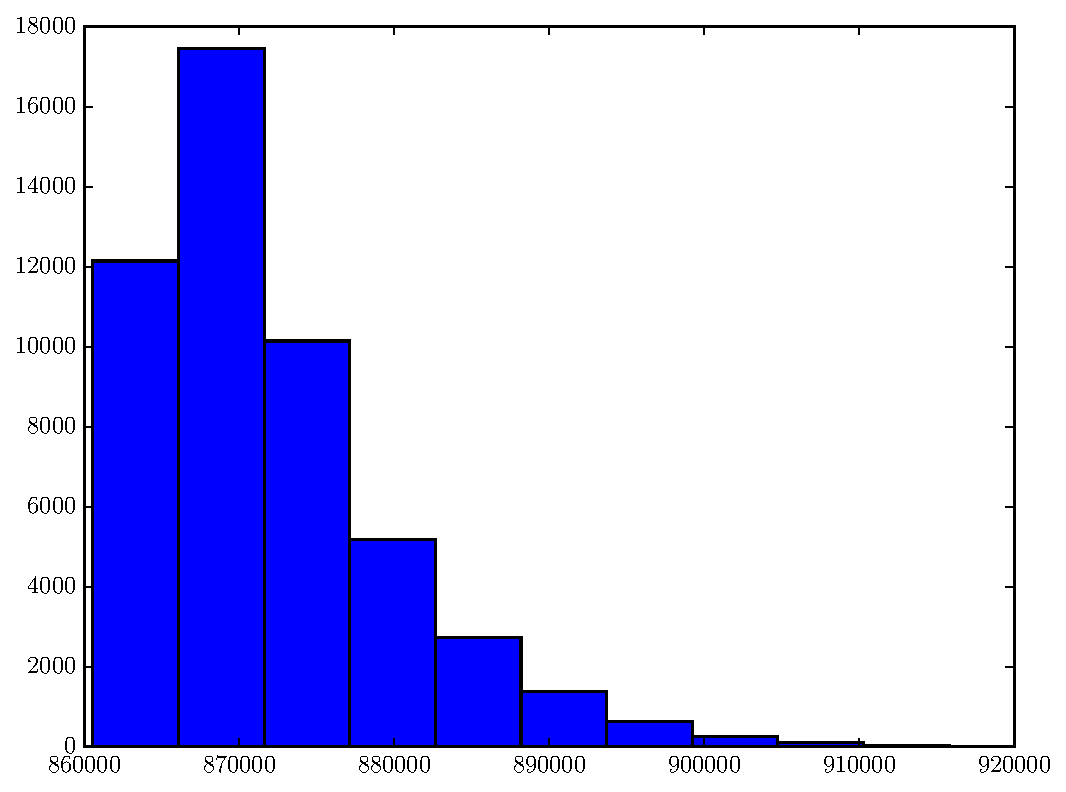
\includegraphics[width=0.3\paperwidth]{../fig/io_hist.pdf}
  \end{subfigure}
  \caption{}
  \label{histos}
\end{figure}

\begin{table}
  \centering
  \caption{}
  \label{iopo_table}
\begin{tabular}{lrrr}
\toprule
{} &         Moyenne &    Écart-Type &   Asymétrie \\
\midrule
IO &  \num{870785}\$ & \num{6734.77} &  \num{1.30} \\
PO & \num{7156512}\$ & \num{2307.67} & \num{-1.07} \\
\bottomrule
\end{tabular}

\end{table}


%%% Local Variables:
%%% mode: latex
%%% TeX-master: "rapport"
%%% End: